% =====================================================================
%  全套提交包 —— 研究报告 + 佐证材料 + 一图流海报 + 答辩幻灯
%  编译：确保 main/evidence/poster/slides.pdf 已生成，再 xelatex 两次
% =====================================================================
\documentclass[a4paper,12pt,fontset=none]{ctexart}
\usepackage[a4paper,margin=2.5cm]{geometry}
\setCJKmainfont{Noto Serif CJK SC}
\setCJKsansfont{Noto Sans CJK SC}
\usepackage{pdfpages}
\usepackage{tikz}
\usepackage{xcolor}
\definecolor{abbred}{RGB}{217,74,31}
\definecolor{abbdark}{RGB}{24,24,24}
\definecolor{abbgray}{RGB}{95,95,95}
\definecolor{abblight}{RGB}{246,242,240}
\pagestyle{empty}

% ---- 统一分隔页 ----
\newcommand{\dividerpage}[3]{%
  \clearpage\thispagestyle{empty}%
  
\begin{tikzpicture}[remember picture,overlay]
    \fill[abbred] (current page.north west) rectangle ([yshift=-1.6cm]current page.north east);
    \fill[abbdark] ([yshift=-1.6cm]current page.north west) rectangle ([yshift=-1.85cm]current page.north east);
    \fill[abblight] (current page.south west) rectangle ([yshift=2.2cm]current page.south east);
  \end{tikzpicture}%
  \vspace*{6cm}
  \begin{center}
  {\sffamily\bfseries\color{abbgray}\Large 人工智能创新赛 · abb-offline-coder}\\[1.2cm]
  {\sffamily\fontsize{40}{46}\selectfont\bfseries\color{abbdark} #1}\\[0.5cm]
  {\color{abbred}\rule{6cm}{2pt}}\\[0.7cm]
  {\sffamily\LARGE\bfseries #2}\\[0.4cm]
  {\large\color{abbgray} #3}
  \end{center}
  \vfill
  \begin{center}{\sffamily\small\color{abbgray}
  队伍：人工智能创新001 \quad|\quad 完全离线 · 中文需求 → ABB RAPID 喷涂程序}\end{center}
  \clearpage}

\begin{document}

% 一、研究报告（含自带封面）

\includepdf[pages=-,fitpaper=true]{main.pdf}

% 二、佐证材料
\dividerpage{附\,录\,A}{项目佐证材料}{可复现实测 · Git 历史 · 单元测试 · 核心能力实跑 · 真实产物}
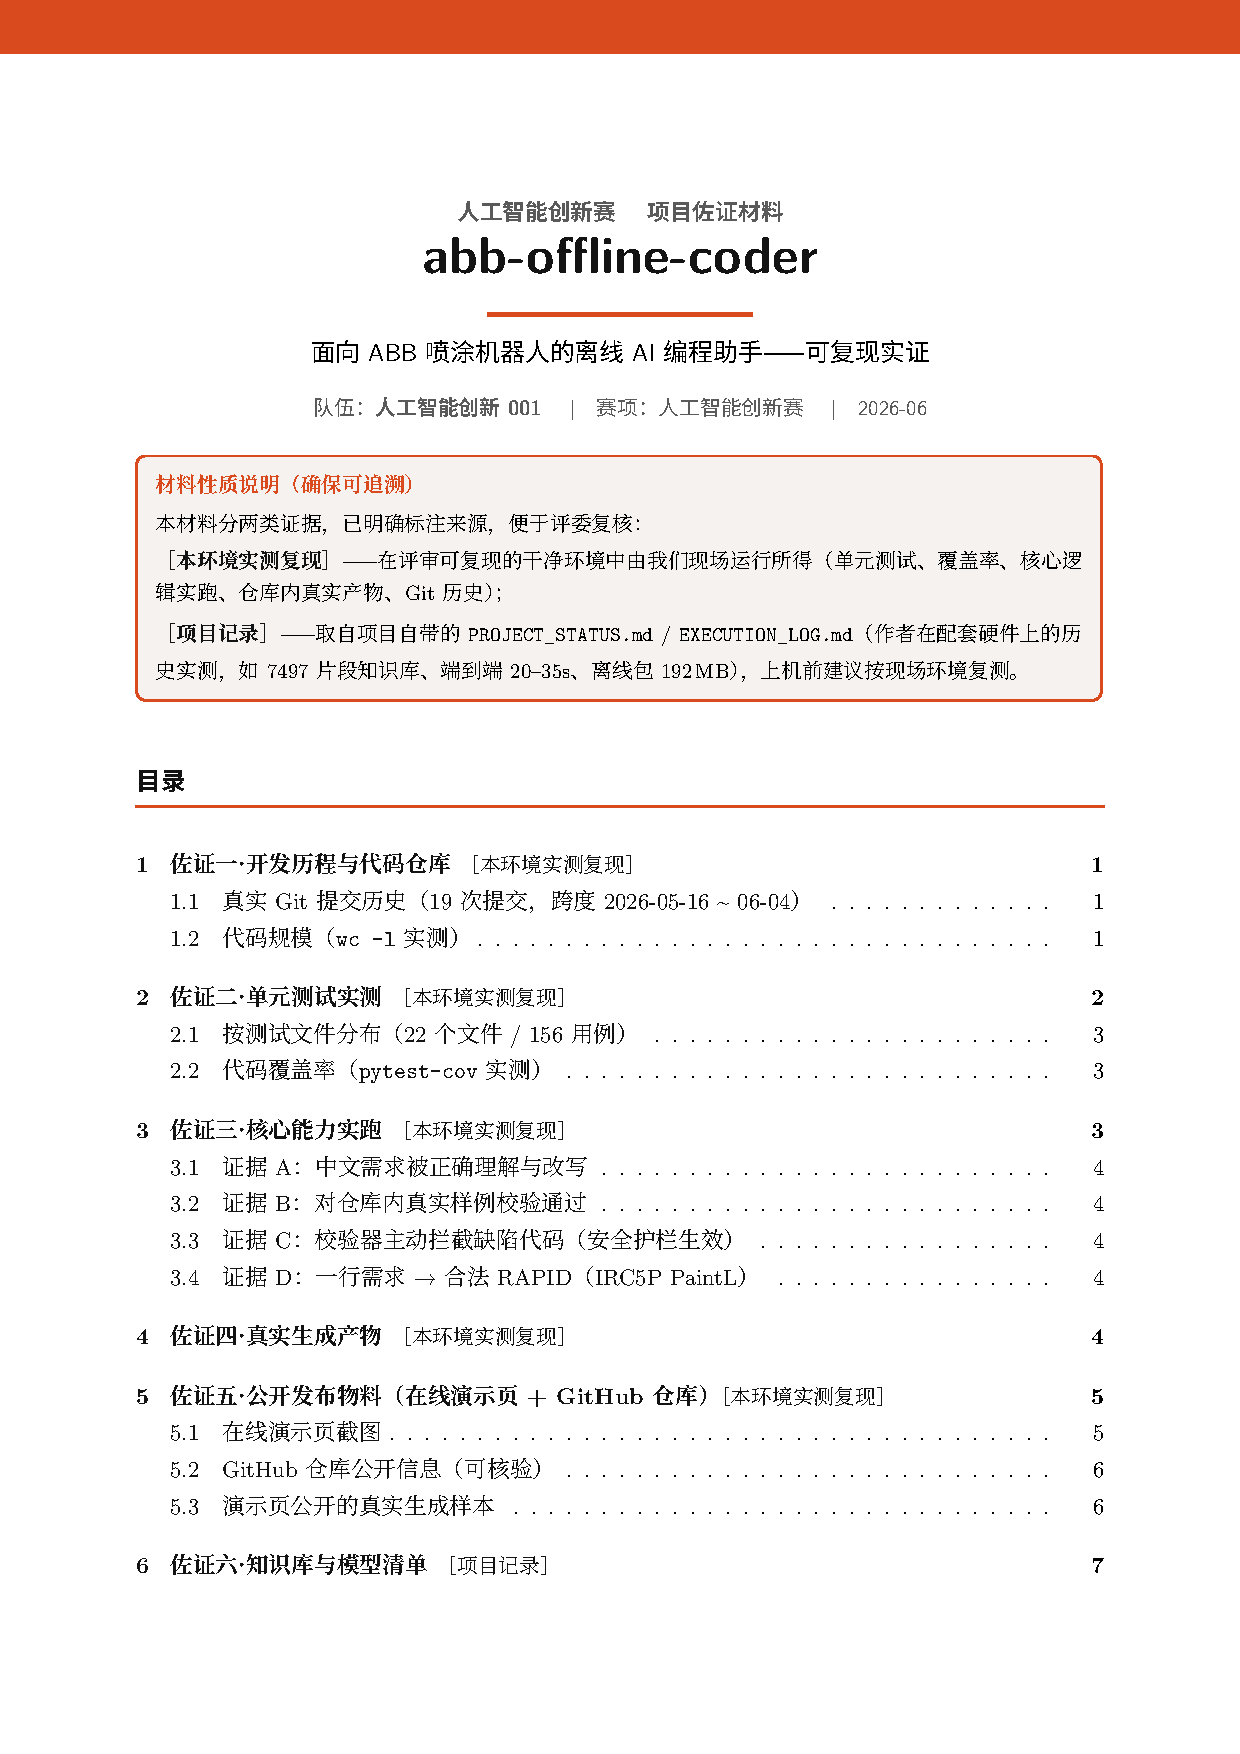
\includepdf[pages=-,fitpaper=true]{evidence.pdf}

% 三、一图流海报（A4 横版）
\dividerpage{附\,录\,B}{项目一图流海报}{答辩展板 / 路演 · 一图速览（A4 横版）}
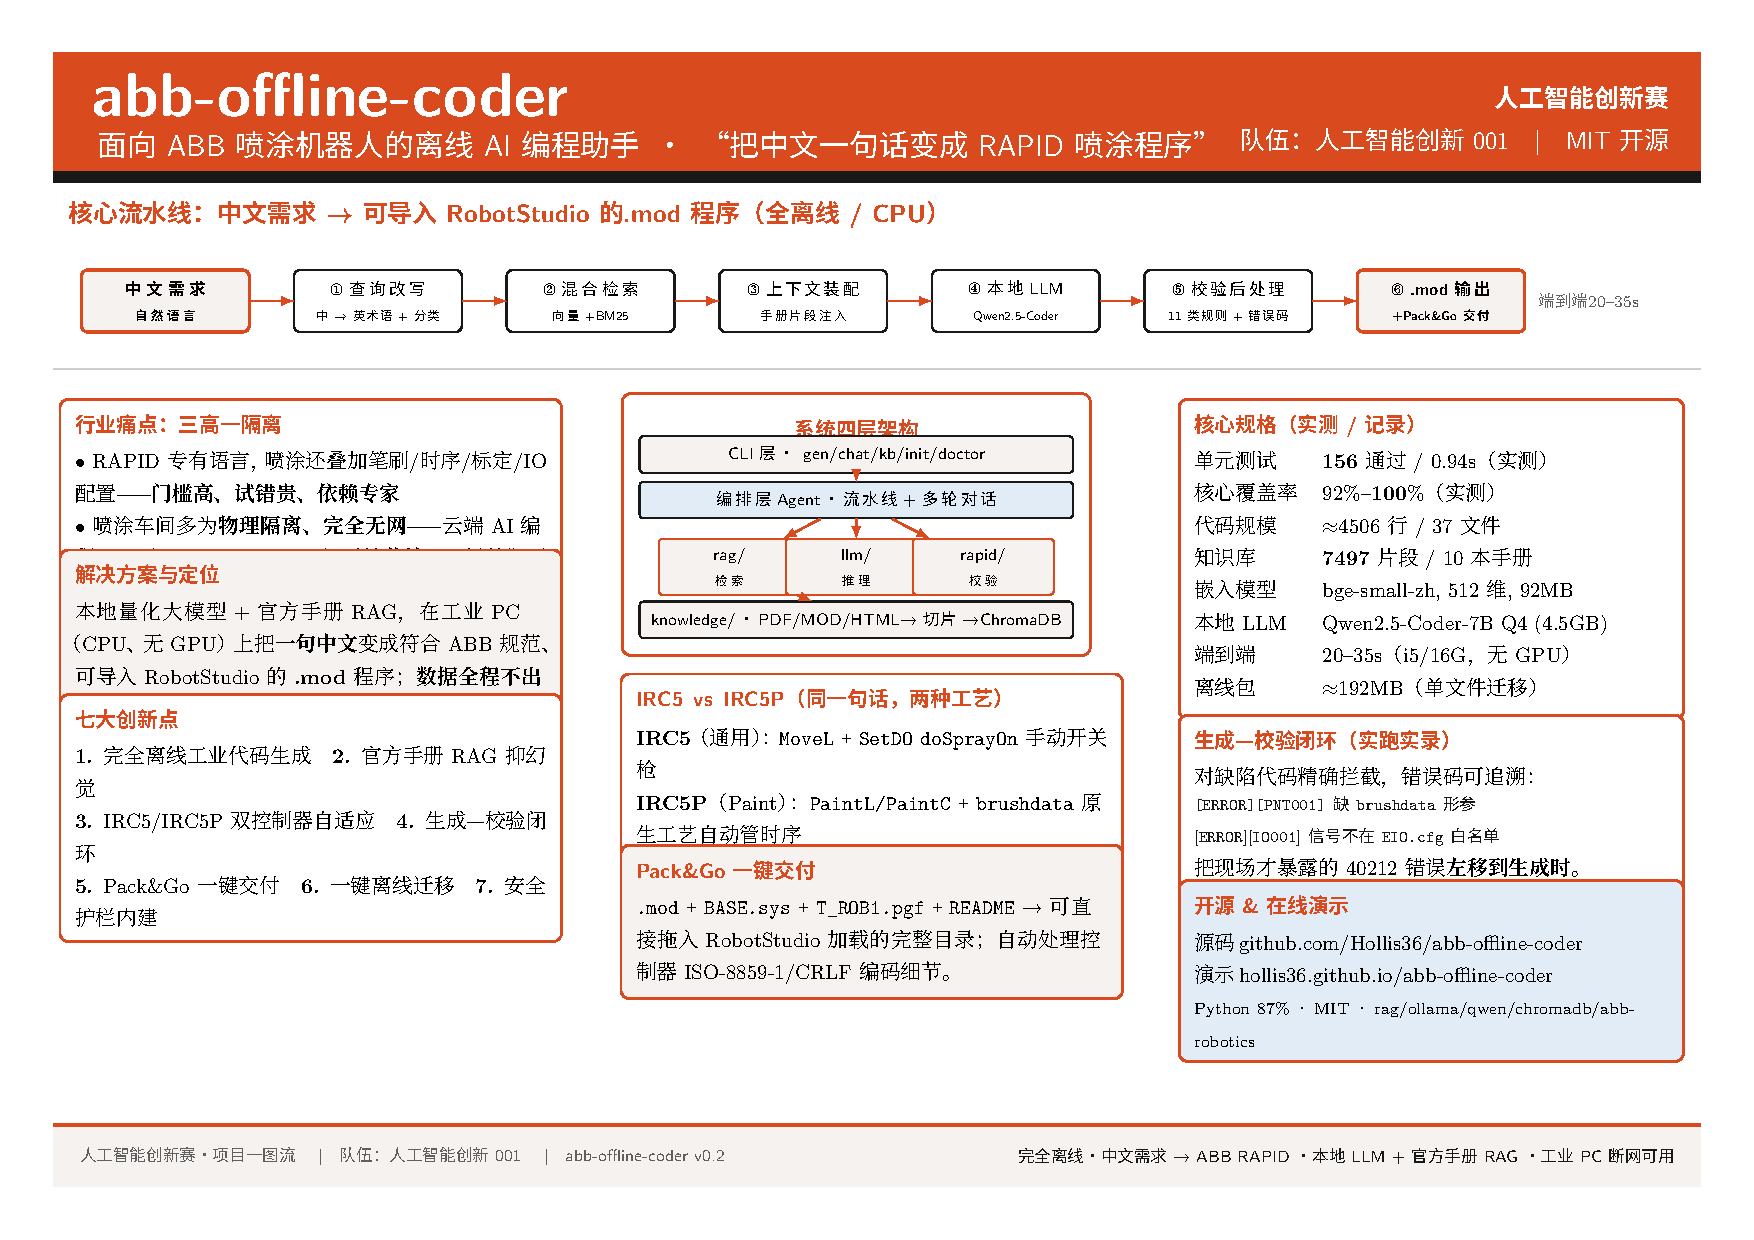
\includepdf[pages=-,fitpaper=true]{poster.pdf}

% 四、答辩幻灯（16:9）
\dividerpage{附\,录\,C}{答辩幻灯}{Beamer 16:9 · 10 页}

\includepdf[pages=-,fitpaper=true]{slides.pdf}

\end{document}
